\documentclass{proposal}

\title{Reversing the reality gap}
\author{Anthony J. Clark, Pomona College, Claremont, CA, USA}
\addbibresource{example-data/example.bib}

\usepackage{fancyhdr}
\usepackage{lastpage}

\pagestyle{fancy}
\fancyhf{}
\renewcommand{\headrulewidth}{0pt}
\cfoot{\footnotesize Project Description---Page \thepage{} of \pageref*{LastPage}}

% \addto\extrasenglish{\def\figureautorefname{Fancy figure}}
% \usepackage{minted}

% Better handling of links
% \usepackage{url}

% Reset page numbering to 1.  This is helpful, since the text can only
% be 15 pages (unless otherwise specified, see individual solicitations),
% and reviewers will want to believe we've kept it within those limits
% \newcommand{\newsection}[1]{\pagenumbering{arabic}\renewcommand{\thepage}{#1--\arabic{page}}}

\begin{document}

\maketitle
\thispagestyle{fancy}

\section{Introduction}
Lorem ipsum dolor sit amet, consectetur adipisicing elit, sed do eiusmod
tempor incididunt ut labore et dolore magna aliqua. Ut enim ad minim veniam,
quis nostrud exercitation ullamco laboris nisi ut aliquip ex ea commodo
consequat. Duis aute irure dolor in reprehenderit in voluptate velit esse
cillum dolore eu fugiat nulla pariatur. Excepteur sint occaecat cupidatat non
proident, sunt in culpa qui officia deserunt mollit anim id est laborum.

\begin{callout}
    The overarching goal of our lab is to develop novel methods for search and exploration. Specifically, we are interested in developing robot learning methods that enable robots to navigate any terrain. To construct devices that operate in rough, unstructured environments we design them with multiple modes of locomotion (e.g., wheeled, flight, walking, etc.). We refer to such robots as adaptive-locomotion robots; they are able to dynamically choose different methods of locomotion at runtime (see Figure 1 for an example). An example application for such a device is aiding first responders looking for victims of a tornado, such as the one that affected our neighboring community (Joplin, Missouri) in 2011.
\end{callout}

Lorem ipsum dolor sit amet, consectetur adipisicing elit, sed do eiusmod
tempor incididunt ut labore et dolore magna aliqua. Ut enim ad minim veniam,
quis nostrud exercitation ullamco laboris nisi ut aliquip ex ea commodo
consequat. Duis aute irure dolor in reprehenderit in voluptate velit esse
cillum dolore eu fugiat nulla pariatur. Excepteur sint occaecat cupidatat non
proident, sunt in culpa qui officia deserunt mollit anim id est laborum.

\subsection{The same thing}
Lorem ipsum dolor sit amet, consectetur adipisicing elit, sed do eiusmod
tempor incididunt ut labore et dolore magna aliqua. Ut enim ad minim veniam,
quis nostrud exercitation ullamco laboris nisi ut aliquip ex ea commodo
consequat. Duis aute irure dolor in reprehenderit in voluptate velit esse
cillum dolore eu fugiat nulla pariatur. Excepteur sint occaecat cupidatat non
proident, sunt in culpa qui officia deserunt mollit anim id est laborum.

\section{Second}
Lorem ipsum dolor sit amet, consectetur adipisicing elit, sed do eiusmod
tempor incididunt ut labore et dolore magna aliqua. Ut enim ad minim veniam,
quis nostrud exercitation ullamco laboris nisi ut aliquip ex ea commodo
consequat. Duis aute irure dolor in reprehenderit in voluptate velit esse
cillum dolore eu fugiat nulla pariatur. Excepteur sint occaecat cupidatat non
proident, sunt in culpa qui officia deserunt mollit anim id est laborum.

\begin{figure}
    \centering
    \subcaptionbox{Robot Prototype\label{fig:application:robot}}{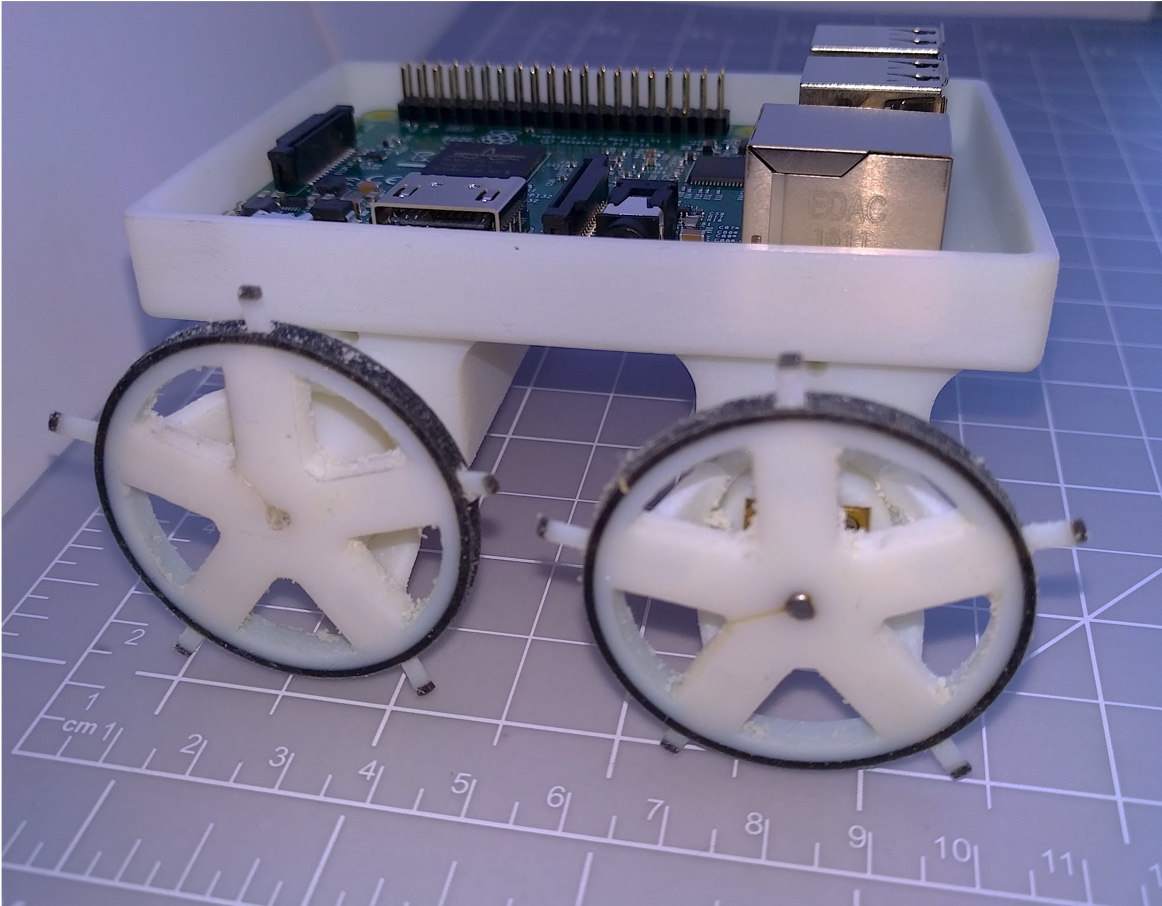
\includegraphics[height=1.55in, frame]{example-data/robot.jpg}}\hfil%
    \subcaptionbox{Application\label{fig:application:env}}{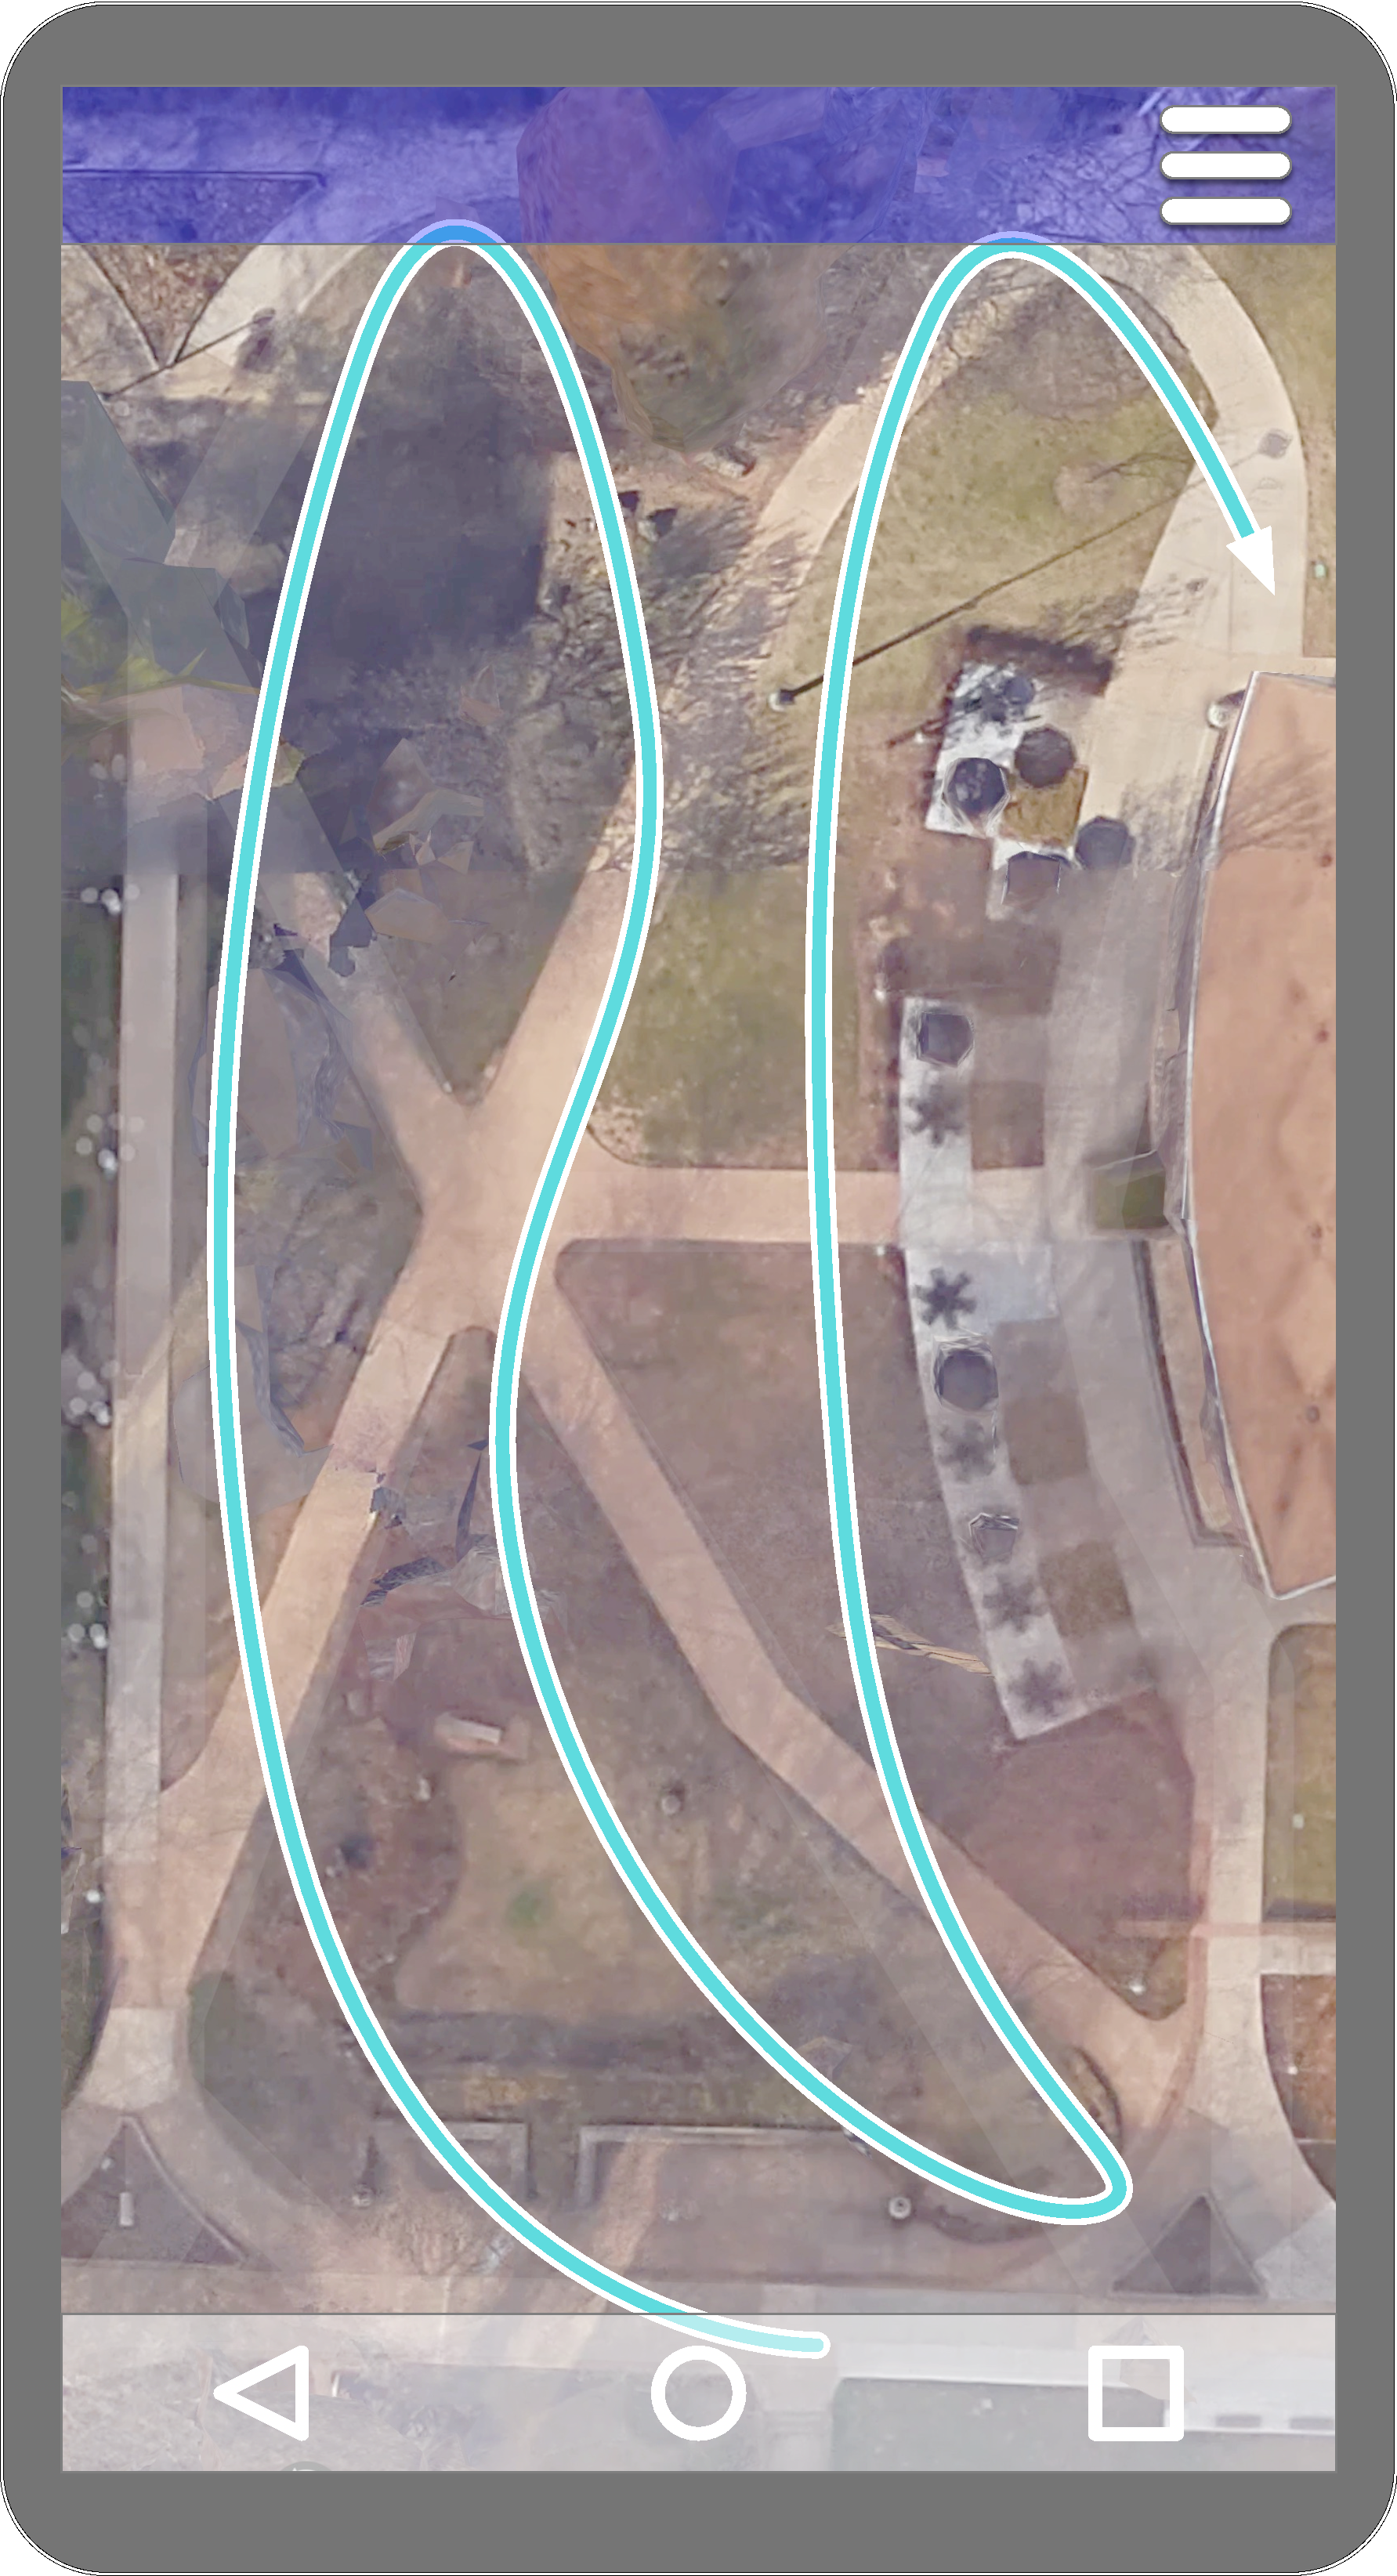
\includegraphics[height=1.55in]{example-data/app.pdf}}\hfil%
    \subcaptionbox{Environment\label{fig:application:app}}{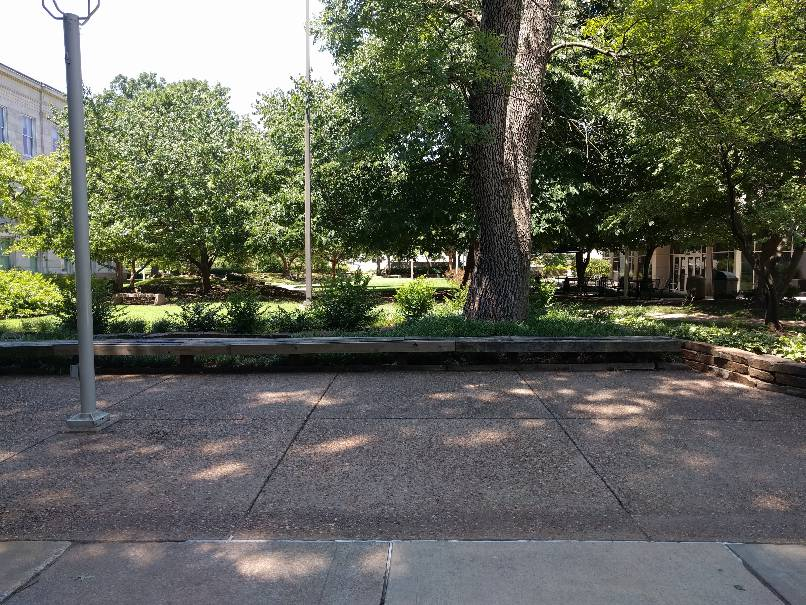
\includegraphics[height=1.55in, frame]{example-data/env.jpg}}
    \caption{(a) Our adaptive-locomotion robot. (b) An example mobile application showing a user-traced path. (c) An area that we would like to search with a semi-autonomous mobile robot.}
    \label{fig:application}
\end{figure}

\paragraph{This is some text}
Lorem ipsum dolor sit amet, consectetur adipisicing elit, sed do eiusmod
tempor incididunt ut labore et dolore magna aliqua. Ut enim ad minim veniam,
quis nostrud exercitation ullamco laboris nisi ut aliquip ex ea commodo
consequat. Duis aute irure dolor in reprehenderit in voluptate velit esse
cillum dolore eu fugiat nulla pariatur. Excepteur sint occaecat cupidatat non
proident, sunt in culpa qui officia deserunt mollit anim id est laborum.~\autoref{fig:application:env}.

This is a citation~\autocite{einstein} and this is a text citation~\textcite{dirac}
... of an enumerated environment that
\begin{linline}
    \item can be used within paragraphs,
    \item takes care of enumeration and
    \item has items that can be referenced.
    \label{lst:test}
\end{linline}
Another posting mentioned ...\autoref{lst:test}

Lorem ipsum dolor sit amet, consectetur adipisicing elit, sed do eiusmod
tempor incididunt ut labore et dolore magna aliqua. Ut enim ad minim veniam,
quis nostrud exercitation ullamco laboris nisi ut aliquip ex ea commodo
consequat. Duis aute irure dolor in reprehenderit in voluptate velit esse
cillum dolore eu fugiat nulla pariatur. Excepteur sint occaecat cupidatat non
proident, sunt in culpa qui officia deserunt mollit anim id est laborum.

Lorem ipsum dolor sit amet, consectetur adipisicing elit, sed do eiusmod
tempor incididunt ut labore et dolore magna aliqua. Ut enim ad minim veniam,
quis nostrud exercitation ullamco laboris nisi ut aliquip ex ea commodo
consequat. Duis aute irure dolor in reprehenderit in voluptate velit esse
cillum dolore eu fugiat nulla pariatur. Excepteur sint occaecat cupidatat non
proident, sunt in culpa qui officia deserunt mollit anim id est laborum.

\printbibliography

\end{document}
